\documentclass{article}
\textwidth=600pt
% Language setting
% Replace `english' with e.g. `spanish' to change the document language
\usepackage[russian]{babel}
% \usepackage[document]{ragged2e}
% Set page size and margins
% Replace `letterpaper' with`a4paper' for UK/EU standard size
\usepackage[letterpaper,top=2cm,bottom=2cm,left=3cm,right=3cm,marginparwidth=1.75cm]{geometry}
\usepackage[strict]{changepage}
\usepackage{indentfirst}
\usepackage{amsmath}
\usepackage{amssymb}
\usepackage{graphicx}
\usepackage{wrapfig}
\usepackage[colorlinks=true, allcolors=blue]{hyperref}

\title{\bf Обзор сложностей некоторых головоломок и настольных игр}
\author{Кунин-Богоявленский Сергей}
\date{16 декабря 2023 г.}
\begin{document}
\maketitle

\begin{abstract}
Данный проект подготовлен для зачета на курсе <<Сложности вычислений>> в МФТИ. \\
Речь идет о вычислительной сложности различных головоломок и игр, показавшихся автору интересными. Также приведено доказательство $\mathbf{NP}$-полноты ребусов определенного типа, именуемых <<криптарифмами>>.
\end{abstract}

\section*{Введение}

Различные игры и головоломки окружают нас с детства. Многие из них интересны своей сложностью --- для решения иной головоломки приходится изрядно поломать голову. Часто эту cложность можно показать математически: каждая $\mathbf{NP}$-полная задача в некотором смысле является головоломкой, и, наоборот, многие головоломки являются $\mathbf{NP}$-полными. Игры для двух игроков обычно имеют более высокую сложность, например, являются $\mathbf{PSPACE}$-полными.

Когда мы говорим о вычислительной сложности таких игр, речь идет не о классических их вариантах, которые, разумеется, лежат в P просто из-за конечности числа каких-либо игровых конфигураций, а об их обобщениях до сколь угодно больших размеров.

Не стоит думать, что эта тема искусственна --- многие ученые всерьез занимаются этим, подтверждением чему является международная конференция <<Fun with Algorithms>>, каждый год привносящая в науку интересные статьи по самым разным играм и головоломкам.


В первую очередь я перечисляю здесь реальные игры и головоломки, которые были изобретены для того, чтобы в них играли, а не анализировали. 

\section*{Игры и головоломки}


\subsection*{Шахматы}

\begin{wrapfigure}[8]{r}{0in}
    \centering
    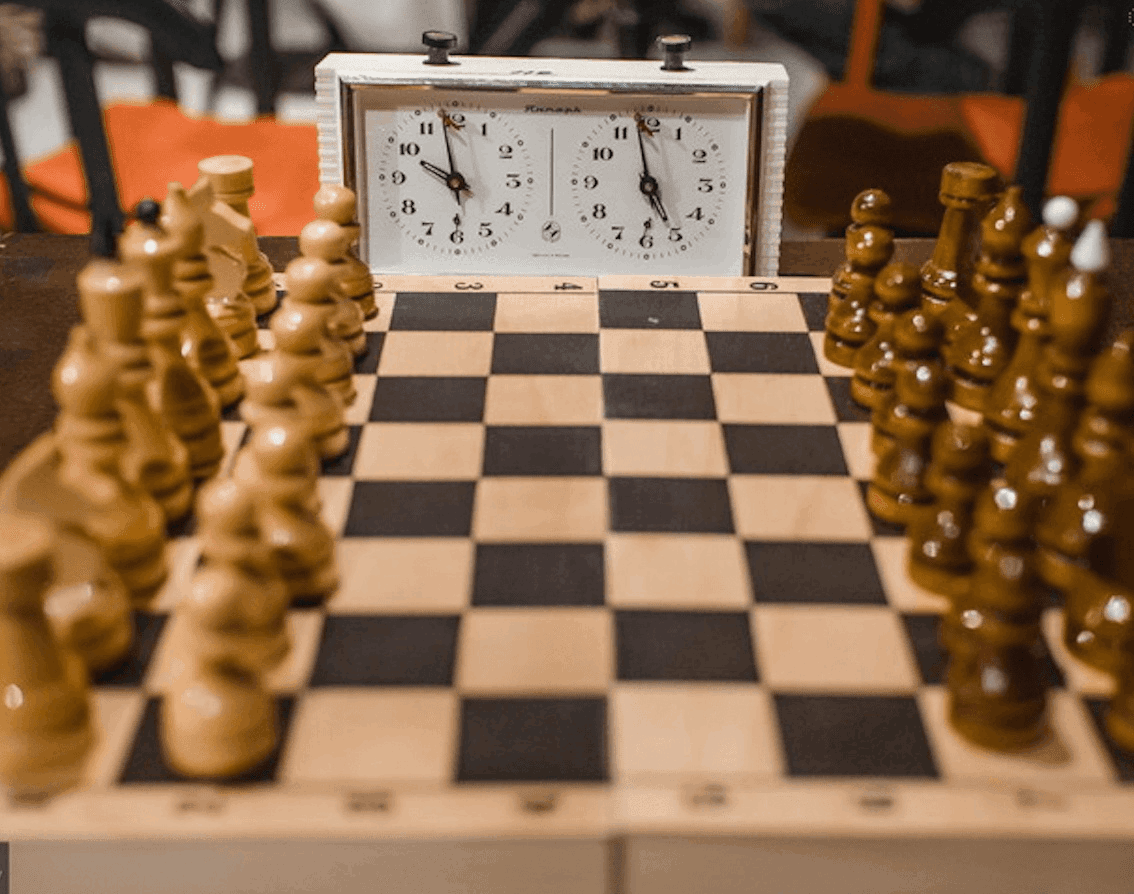
\includegraphics[width=0.2\textwidth]{chess.jpg}
    \caption{Шахматы}
\end{wrapfigure}

\noindent\textit{\underline{Описание:}} Надеюсь, не нуждается в представлении, но основная идея состоит в том, чтобы передвигать фигуры по доске $8 \times 8$, захватывая фигуры своих противников, до тех пор, пока игра не закончится или матом, или различными видами ничьих \\

\noindent\textit{\underline{Сложность:}} Классический вариант конечен, но обобщение дo $n \times n$ $\mathbf{PSPACE}$-полно c <<правилом 50-ти ходов>>, и $\mathbf{EXP}$-полно --- без него \cite{chess}.
\newpage

% \subsection*{Шашки}

% \begin{wrapfigure}[4]{l}{0in}
%     \centering
%     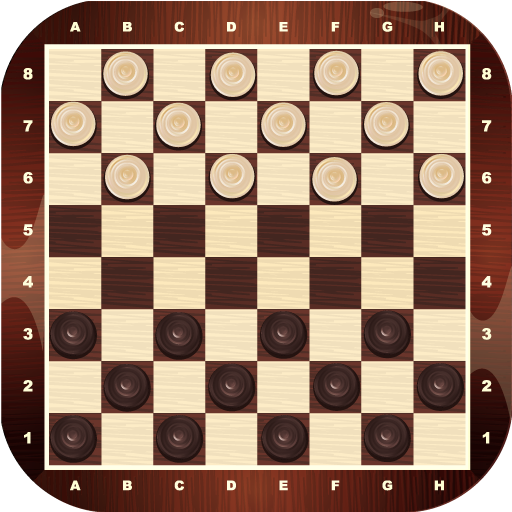
\includegraphics[width=0.16\textwidth]{checkers.png}
%     \caption{Шашки}
% \end{wrapfigure}
% \frenchspacing
% \textit{\underline{Описание:} } Игроки поочердно перемещают шашки на одну клетку по диагонали на чередующихся клетках доски $n \times n$, съедая фигуры  других игроков по диагонали. Цель --- оставить противника без хода. 
% \\

% \noindent\textit{\underline{Сложность:}} $\mathbf{EXP}$-полная.

% \vspace*{0.7in}

\subsection*{Реверси}

\begin{wrapfigure}[8]{l}{0in}
    \centering
    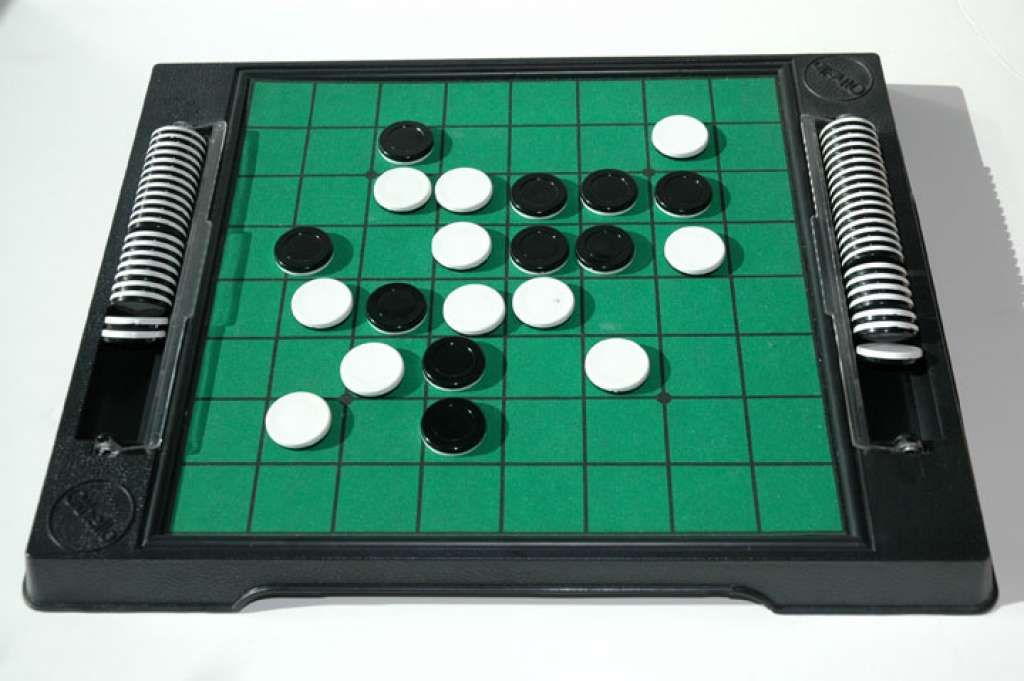
\includegraphics[width=0.24\textwidth]{reversi.jpg}
    \caption{Реверси}
\end{wrapfigure}
\frenchspacing
\noindent \textit{\underline{Описание:} } Играют двусторонними фишками на квадратной доске. Игроки поочередно размещают фишки на доске своим цветом вверх, переворачивая фишки цвета противника, зажатые между новой и старой фишкой своего цвета, захватывая таким образом отрезок. Цель  --- к концу игры занять своим цветом больше полей, чем противник.
\\

\noindent\textit{\underline{Сложность:}} Обобщенная на $n \times n$, $\mathbf{PSPACE}$-полна \cite{othello}.

\vspace*{0.3in}

% \subsection*{Криптарифмы}

% \begin{wrapfigure}[4]{r}{0in}
%     \centering
%     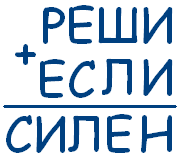
\includegraphics[width=0.15\textwidth]{cryptarithm.png}
%     \caption{Ребус}
% \end{wrapfigure}

% \textit{\underline{Описание:}} В этих головоломках последовательность букв упорядочена в виде примера сложения в столбик. Задача заключается в том, чтобы построить биекцию между буквами и цифрами, в результате которой получится корректный пример. \\

% \noindent\textit{\underline{Сложность:}} Обобщения на $n$-ичные основания $\mathbf{NP}$-полны.

\subsection*{Пятнашки}

\begin{wrapfigure}[7]{r}{0in}
    \centering
    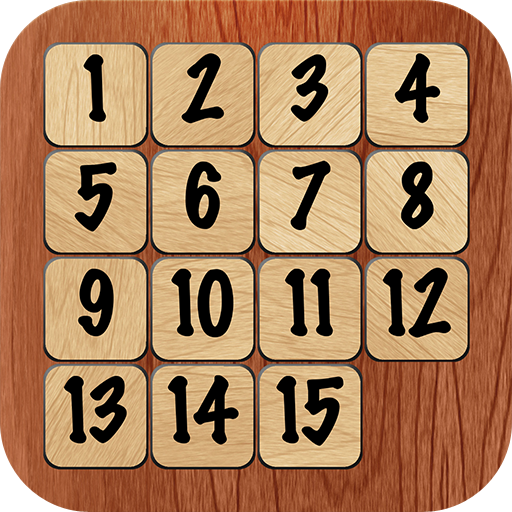
\includegraphics[width=0.18\textwidth]{15puzzle.png}
    \caption{Пятнашки}
\end{wrapfigure}


\noindent\textit{\underline{Описание:}} В матрице $4 \times 4$ все поля, за исключением одного, заняты фишками. Фишки, примыкающие к пустому полю, могут быть сдвинуты на его место. Цель заключается в том, чтобы добиться определенной перестановки фишек. \\

\noindent\textit{\underline{Сложность:}} Классика конечна, но легко обобщается до $n \times n$. Проверка того, существует ли решение, находится в $\mathbf{P}$, но поиск решения с наименьшим количеством ходов является $\mathbf{NP}$-полным \cite{fifteen}.

\vspace*{0.3in}

\subsection*{Японские кроссворды}

\begin{wrapfigure}[9]{l}{0in}
    \centering
    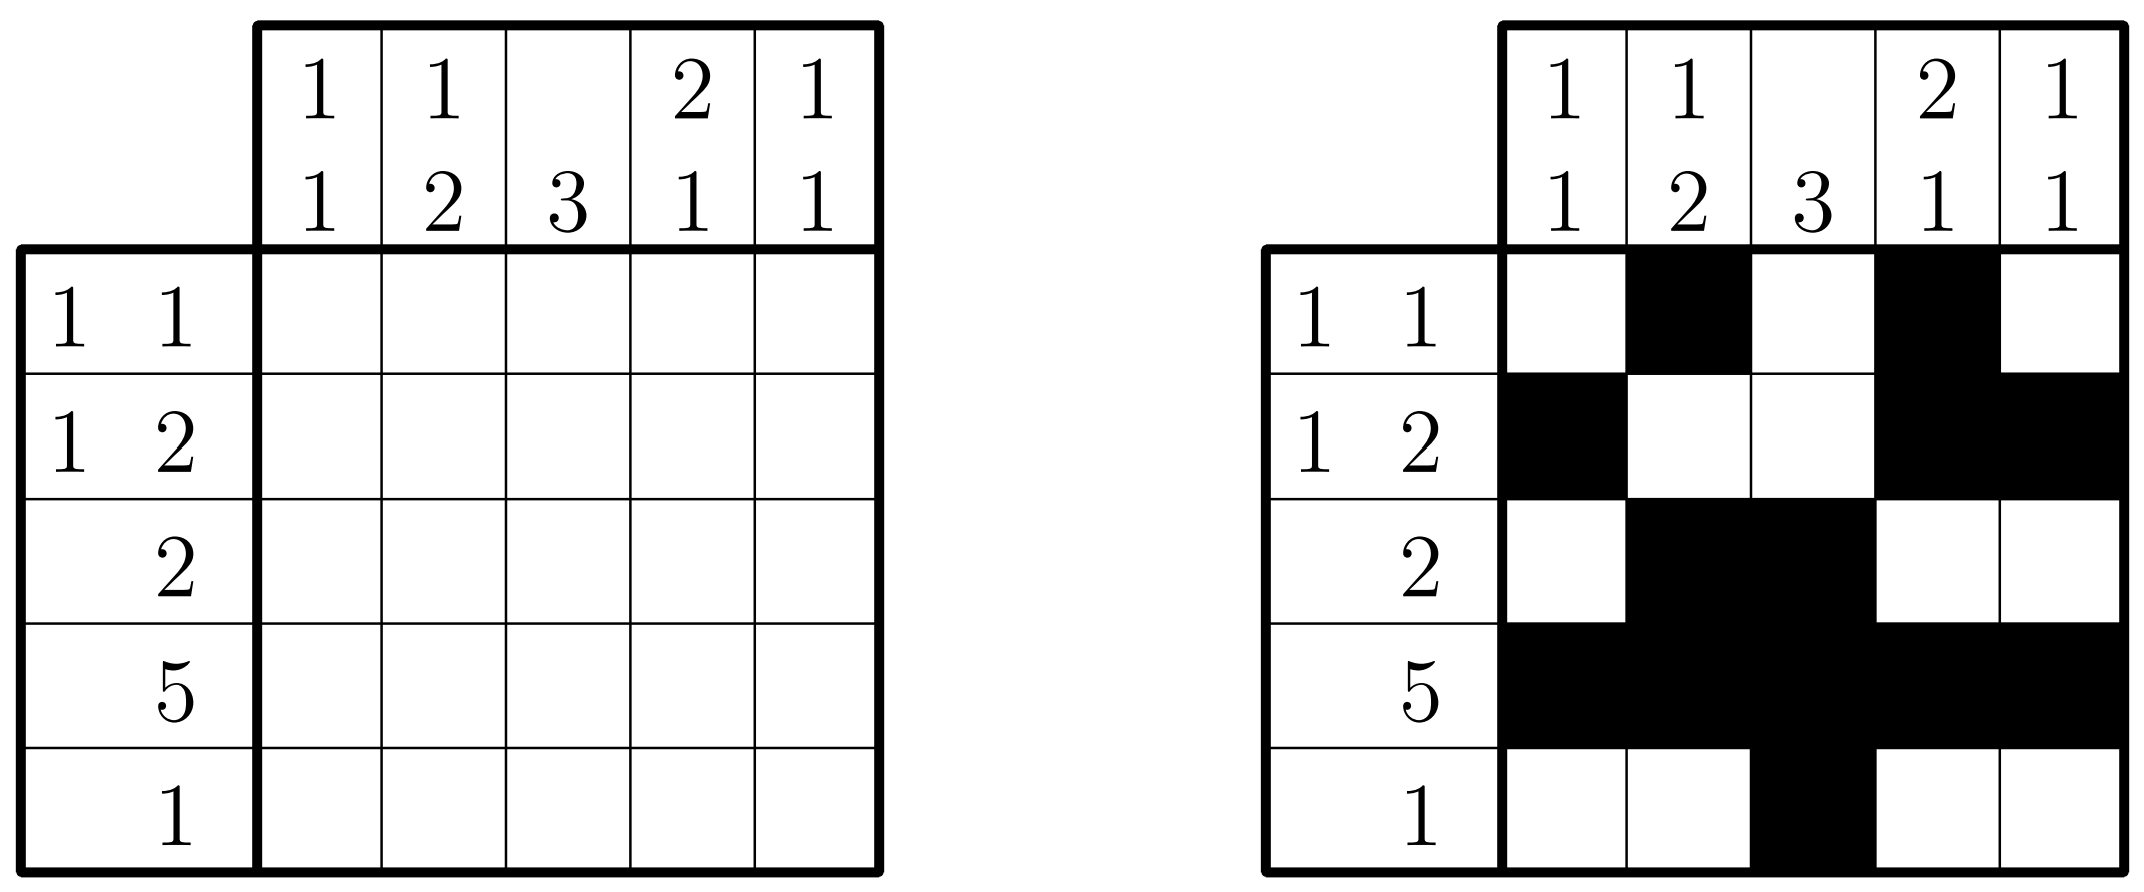
\includegraphics[width=0.4\textwidth]{nonogram.jpg}
    \caption{Решение японского кроссворда}
\end{wrapfigure}

\noindent\textit{\underline{Описание:}} Изображение закодировано числами по строкам и по столбцам. Количество чисел показывает, сколько групп чёрных клеток находятся в соответствующих строке или столбце, а сами числа — сколько слитных клеток содержит каждая из этих групп. Необходимо определить размещение черных клеток. \\

\noindent\textit{\underline{Сложность:}} $\mathbf{NP}$-полна \cite{nonograms}.

\vspace*{0.3in}

\subsection*{Го}

\begin{wrapfigure}[7]{r}{0in}
    \centering
    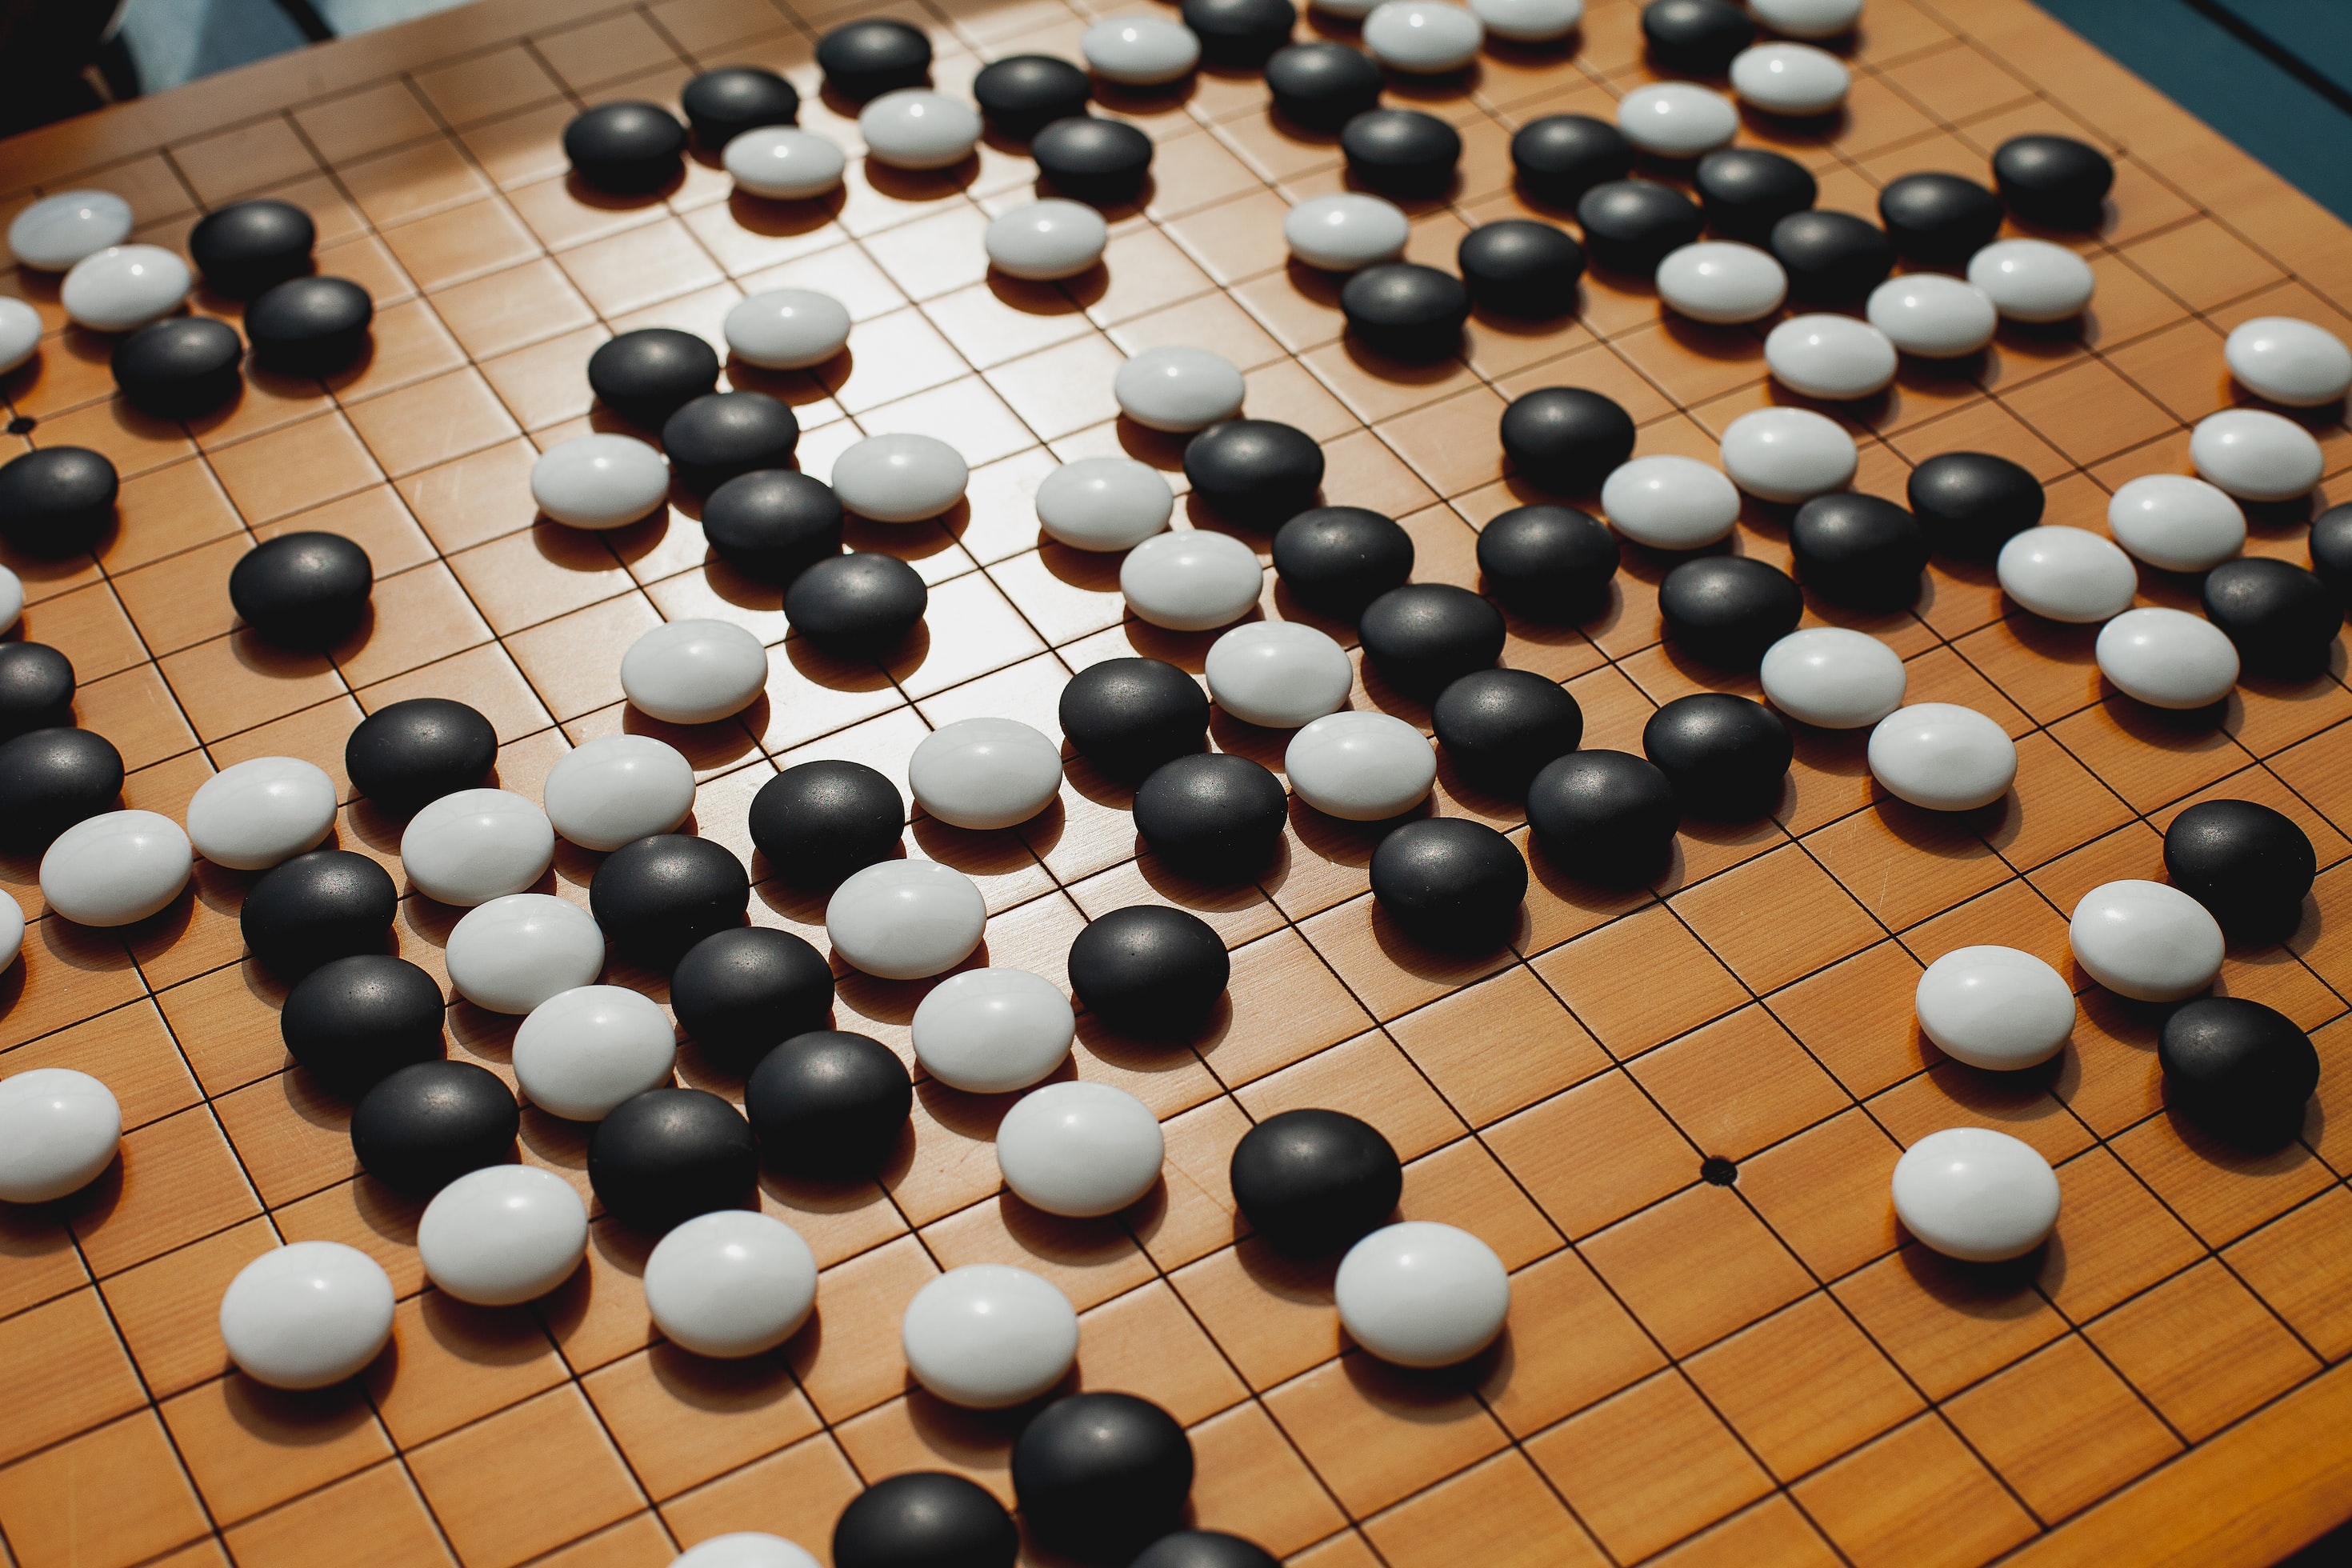
\includegraphics[width=0.25\textwidth]{go.jpeg}
    \caption{Го}
\end{wrapfigure}

\noindent\textit{\underline{Описание:}} Игра на доске размером $19\times19$.
Суть заключается в том, что нужно отгородить на игровой доске камнями своего цвета большую территорию, чем противник. \\

\noindent\textit{\underline{Сложность:}} Обобщение до $n \times n$ $\mathbf{PSPACE}$-полно. Вариация игры с $ko$-правилом (запретом повторения позиции на следующем ходу) $\mathbf{EXP}$-полна \cite{go}. 

% \clearpage

\subsection*{Криптарифмы}

\begin{wrapfigure}[6]{l}{0in}
    \centering
    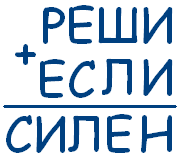
\includegraphics[width=0.15\textwidth]{cryptarithm.png}
    \caption{Ребус}
\end{wrapfigure}

\noindent\textit{\underline{Описание:}} В этих головоломках последовательность букв упорядочена в виде примера сложения в столбик. Задача заключается в том, чтобы построить биекцию между буквами и цифрами, в результате которой получится корректный пример. \\

\noindent\textit{\underline{Сложность:}} Обобщения на $n$-ичные основания $\mathbf{NP}$-полны.

\section*{$\mathbf{NP}$-полнота языка $\mathsf{CRYPTA}$\footnote{Доказательство основано на материале Дэвида Эпштейна \cite{cryptarithms}}}

Мы докажем, что язык $\mathsf{CRYPTA}$, состоящий из множества корректных разрешимых криптарифмов, является $\mathbf{NP}$-полным. \\

\subsection*{\underline{Принадлежность $\mathbf{NP}$}}
Тривиально, в качестве сертификата посылается строка, задающая биекцию между алфавитом криптарифма и неотрицательными целыми числами меньше основания.  \\
Проверка корректности сложения выполняется за полином.

\subsection*{\underline{$\mathbf{NP}$ - трудность}}
Верно следующее: $3\mathsf{SAT} \leq_p \mathsf{CRYPTA}$ \\

% Пусть формула $\varphi \in 3\mathsf{SAT}$
Для доказательства сводимости нам необходимо предъявить полиномиально вычислимую функцию $F$, такую что $\forall \varphi \quad \varphi \in 3\mathsf{SAT} \Leftrightarrow  F(\varphi) \in \mathsf{CRYPTA}$

\subsubsection*{\textit{Построение криптарифма}}
Первым делом обязательно отдадим крайние правые три столбца под следующую конструкцию (\textit{см. слева}):

$$
  \begin{array} {c*{3}{@{\ }c}}
     k & p & k \\ 
     k & p & k \\
     \hline
     l & q & k
  \end{array}
  \qquad
  \Longrightarrow
  \qquad
  % \longrightarrow
  \begin{array} {c*{3}{@{\ }c}}
     0 & p & 0 \\ 
     0 & p & 0 \\
     \hline
     1 & q & 0
  \end{array}
$$

 \par Для верности этой части критарифма необходимо, чтобы $k = 0$ и $l = 1$ (действительно, единственное значение $k$, при котором $2k\ \%\ n = k$ --- это 0, откуда из невозможности соответствия разным буквам одного числа следует, что на третий разряд происходит перенос, и это дает $l$ значение $1$). Таким образом, мы сразу зарезервировали буквы $k$ и $l$, поэтому для простоты дальнейшем будем вместо них писать сразу $0$ и $1$ соответственно.

\indent Теперь обратим свой взор на литералы и их отрицания. Следующая конструкция
\newline

\begin{center}
\begin{tabular}{c*{13}{@{\ }c}}
 $d_i$ & 0 & 1 & $y_i$ & 0 & $c_i$ & $y_i$ & 0 & $b_i$ & $y_i$ & 0 & $a_i$ & 0 \\ 
$e_i$ & 0 & $d_i$ & $y_i$ & 0 & $c_i$ & $y_i$ & 0 & $b_i$ & $y_i$ & 0 & $a_i$ & 0 \\
 \hline
 $\overline{v_i}$ & 0 & $e_i$ & $z_i$ & 0 & $d_i$ & $z_i$ & 0 & $v_i$ & $z_i$ & 0 & $b_i$ & 0    
\end{tabular}
\end{center}

\noindent обязывает буквы $v_i$ и $\overline{v_i}$ быть по модулю 4 равными 0 и 1 или наоборот. В самом деле, $b_i$ точно четно как $2a_i$, поэтому $v_i$ равно либо $4a_i$, либо $4a_i+1$. В первом случае переноса при суммировании $y_i$ не происходит, а значит $d_i = 2c_i$, $e_i = 2c_i + 1$, $\overline{v_i} = 4c_i + 1$. Во втором случае аналогичными умозаключениями, но уже с переносом, получается  $\overline{v_i} = 4c_i + 4$.
Раз так, скажем, что $v_i$ соответствует булевой истине, если по модулю 4 оно равно 1, и булевой лжи --- в случае 0, а  $\overline{v_i}$ есть её отрицание.

Наконец, в 3-КНФ формуле $\varphi$ будут дизъюнкты вида $v_a \vee v_b \vee v_c$. Для них соорудим следующую конструкцию (для дизъюнкта $v_a \vee v_b \vee v_d$ нужно будет использовать ту же $u_{ab}$, что здесь)

\begin{center}
\begin{tabular}{c*{12}{@{\ }c}}
 $u_{ab}$ & 0 & $v_a$ & 0 & $1$ & $r_i$ & 0 & $g_i$ & $w_i$ & 0 & $f_i$ & 0 \\ 
$v_c$ & 0 & $v_b$ & 0 & $h_i$ & $r_i$ & 0 & $g_i$ & $w_i$ & 0 & $f_i$ & 0 \\
 \hline
 $t_i$ & 0 & $u_{ab}$ & 0 & $t_i$ & $s_i$ & 0 & $h_i$ & $x_i$ & 0 & $g_i$ & 0    
\end{tabular}
\end{center}

\noindent Тут можно заметить, что $h_i$ по модулю 4 равна либо 0, либо 1, а $t_i$ равна либо $h_i + 1$, либо $h_i + 2$. Таким образом, $t_i$ по модулю 4 может принимать значения $1, 2, 3$ $-$ и только их.
С другой стороны, $t_i = v_a + v_b + v_c$, каждая из которых по модулю 4 может принимать лишь 0 и 1 (предыдущую конструкцию мы соорудили для каждого литерала). Таким образом, $t_i$ обязывает хотя бы одну из переменных $v_a, v_b, v_c$ быть истинной -- чего мы и хотим от дизъюнкта.

Итак, созданные ограничения гарантируют противоположные значения литералу и его отрицанию, а также истинность каждого дизъюнкта. Значит, решение криптарифма $F(\varphi)$  дает решение формулы $\varphi$. Это будет верно для любого основания нашего криптарифма. Однако нам также необходима возможность обратной операции --- по разрешимой $\varphi$ получить разрешимую $F(\varphi)$.
Оказывается, при выборе основания, равного $3072n^3$, где $n$ -- число переменных в формуле $\varphi$, можно обеспечить и это.

\subsubsection*{\textit{Разрешение криптарифма}}

Возьмем основание, кратное $128$, и сопоставим буквам следующие значения по модулю $128$:
\vspace{0.1in}
\begin{adjustwidth}{-1in}{-1in}
\begin{center}
\begin{tabular}{|*{14}{l|}}
\hline
Буква: &$a$ & $b$ & $c$ & $d$ & $e$ & $f$ & $g$ & $h$ & $v, \overline{v}$ & $u$ & $t$ & $p, r, w, y$ & $q,s,x,z$  \\
\hline 
Значение: & $2,34$ & $4,68$ & $1,2,33,34$ & $3,4$ & $5,69$ & $6,38$ & $12,76$ & $24,25$ & $8,9$ & $16,17$ & $25,26$ & $7,71$ & $14$ \\
& $66,98$ & & $65,66,97,98$ & $67,68$ & & $70,102$ & & & & $18$ & $27$ & &  \\
\hline 
\end{tabular}
\end{center}
\end{adjustwidth}
\vspace{0.1in}
\noindent Каждой переменной $x$ сопоставим класс $\left \lceil\dfrac{x}{128}\right \rceil $. Нужно чтобы у каждого экземпляра построенных выше конструкций был свой класс, и они не пересекались.

\noindent Можно заметить, что при сложении вида $y+y+carry=x$ значение $y$ определется так: $y$ = $\left \lfloor\dfrac{x}{2}\right \rfloor$. Поэтому при заданных $v$ и $\overline{v}$ все остальные буквы, кроме последних двух столбцов таблички, будут определены однозначно. С заданием букв из этих столбцов проблем также не возникнет, мы выберем из возможных вариантов нужный в зависимости от того, нужен ли перенос.

Оставшаяся проблема --- ситуация, при которой букве необходимо присвоить значение, превосходящее основание криптарифма. Это решается выбором основания, большего чем утроенное максимальное значение, присвоенное переменным вида $v$ (так как самая большая из задаваемых ими букв $t_i$ будет cуммой $v_a$, $v_b$, $v_c$).

Таким образом, наша задача свелась к тому, чтобы присвоить классам переменных $v_i$ такие значения, чтобы суммы всевозможных троек из них не пересекались. Если у нас это получится, мы, в соответствии с таблицей, выберем для $v_i$ остаток $8$ или $9$ по модуля $128$ в зависимости от истинности или ложности переменной в формуле, и это задаст значения остальных букв.

Здесь мы воспользуемся результатом \cite{theory_of_numbers}. Доказано, что для любого $k$ между $1$ и $k^3$ найдется множество из $k$ чисел, таких что суммы всевозможных троек различны. Поэтому достаточно, чтобы наши классы пробегали между $1$ и $(2n)^3$. Умножив на 128 $\cdot$ 3, чтобы все буквы вместились, получим $3072n^3$ - достаточный размер основания, при котором все буквы вместятся без поворений. То есть мы доказали и то, что по разрешимой формуле можно за полином построить и разрешимый криптарифм. $\mathbf{NP}$-полнота доказана.


\bibliographystyle{plain} 
\bibliography{refs.bib} 

\end{document}